\subsection{Formulasi Masalah}
\label{subsec:omm-preliminaries}
Sekuens data dari sejumlah K data titik GPS yang dikumpulkan oleh kendaraan didefinisikan dengan \textit{trajectory} $g_{1:K}$. Setiap data titik GPS memiliki data $(g_k.t,g_k.lat,g_k.lng,g_k.v)$ yang secara berturut-turut adalah waktu pengambilan titik GPS, \textit{latitude}, \textit{longitude}, dan kecepatan. Kecepatan dapat diambil dari diferensial antara dua titik GPS. Jaringan jalan adalah sebuah graf berarah $G(V,E)$ dimana $V$ adalah himpunan dari simpul-simpul dan $E$ adalah himpunan dari sisi-sisi yang merepresentasikan segmen jalan. Setiap segmen jalan $e\in E$ memiliki 4 data $(e.id, e.l, e.start, e.end)$ yang secara berturut-turut adalah ID, panjang, titik awal, dan titik akhir dari sisi $e$. Diberikan sebuah rute $r_{1:k}$ adalah sekuens dari sejumlah K segmen-segmen jalan yang sesuai dengan lintasan yang diberikan \textit{trajectory} $g_{1:k}$. Setiap segmen jalan $r_k\in E$ merepresentasikan segmen jalan dimana kendaraan sedang berada pada \textit{time step} $k$. \textit{Online map matching} bertugas untuk menentukan segmen jalan $r_k$ pada setiap \textit{time step} $1\leq k \leq K$ dengan hanya menggunakan titik-titik GPS terdahulu $\{g_i\mid 1\leq i\leq k\}$. Rute $\tau$ adalah rute yang dimulai dari segmen jalan $r_k$ yang mempunyai panjang tak hingga. $\tau$ adalah sekuens dari segmen-segmen jalan yang saling terhubung $\tau=\{e_1\rightarrow e_2\ldots\}, 1 \leq i \leq \infty, \text{ dimana } e_1=r_k, e_i.end=e_{i+1}.start$. Probabilitas rute $\tau$ didefinisikan dengan:
\begin{equation}
    p(\tau)=\prod_{i=1}^{\infty}p(e_i\rightarrow e_{i+1})
\end{equation}

\textit{Online map-matching} dapat dilakukan dengan menggunakan \textit{Bayesian filtering} \cite{Taguchi2019}. \textit{Bayesian filtering} memberikan estimasi probabilitas posterior $p(r_k\mid g_{1:k})$ untuk setiap langkah pengambilan sampel $k$. Probabilitas posterior dapat dihitung melalui teorema bayes sebagai berikut:
\begin{equation}
    p(r_k\mid g_{1:k})=\frac{p(g_k\mid r_k,g_{1:k-1})p(r_k,g_{1:k-1})}{p(g_k\mid g_{1:k-1})}
\end{equation}
Dengan mengasumsikan independensi bersyarat,$g_k \perp\!\!\!\perp g_{1:k-1} \mid r_k $ posterior dapat dihitung dengan:

\begin{align}
p(r_k \mid g_{1:k}) 
&\propto p(g_k \mid r_k)\, p(r_k \mid g_{1:k-1}) \notag\\
&\propto p(g_k \mid r_k) \sum_{r_{k-1}} p(r_k \mid r_{k-1}) \, p(r_{k-1} \mid g_{1:k-1})
\label{eq:bayesian-filtering}
\end{align}

\textit{Bayesian filtering} terdiri dari \textit{prediction} dan \textit{filtering}. \textit{Prediction} menghitung probabilitas \textit{prior} $p(r_k \mid g_{1:k-1})$. $p(r_k\mid r_{k-1})$ adalah probabilitas \textit{route prediction}, yang merepresentasikan probabilitas kendaraan berada di segmen jalan $r_k$ pada langkah waktu berikutnya, berdasarkan segmen jalan sebelumnya. \textit{Filtering} menghitung probabilitas posterior. \textit{Bayesian filtering-based map-matching} melibatkan prosedur \textit{prediction} dan prosedur \textit{filtering} secara berulang. Probabilitas GPS \textit{observation} $p(g_k \mid r_k)$ memberikan \textit{likelihood} bahwa pengukuran GPS $g_k$ dihasilkan ketika kendaraan berada pada segmen jalan $r_k$. \textit{Measurement error} $\lVert g_k-x\rVert_{euclidean}$ diasumsikan mengikuti distribusi Gaussian dengan rata-rata sama dengan nol. Jarak $\lVert \cdot \rVert_{euclidean}$ adalah jarak \textit{euclidean} dari titik hasil proyeksi \textit{equirectangular} dari titik koordinat \textit{latitude} $\phi$  dan \textit{longitude} $\lambda$ \ GPS. Probabilitas GPS \textit{observation} didefinisikan dengan:

\begin{align}
\lVert g_k - x \rVert_{\text{euclidean}} &\sim \mathcal{N}(0,\sigma_g) \notag \\
p(g_k \mid r_k) &= \int_{0}^{r_k.l} p(g_k,x \mid r_k)\, dx \notag  \\
&= \int_{0}^{r_k.l} p(g_k \mid x, r_k)\, p(x \mid r_k)\, dx \notag  \\
&= \int_{0}^{r_k.l} \frac{1}{\sqrt{2\pi\sigma_g}}
    \exp \left(-\frac{\lVert g_k - x \rVert_{\text{euclidean}}^2}{2\sigma_g} \right)
    p(x \mid r_k)\, dx \tag{3.4}\\
\lVert g_k - x \rVert_{\text{euclidean}} 
&= R\sqrt{\bigl((\lambda_{g_k}-\lambda_{x})\cos\phi_m\bigr)^2+(\phi_{g_k}-\phi_{x})^2} \tag{3.5} \\
R &= \text{\textit{equatorial radius} dari Bumi (WGS84)} = 6,378,137 \ \text{m}\notag  \\ 
\phi_m &= 36^\circ \notag \\
x\mid r_k &\sim U(0,r_k.l) \notag \\ 
p(x\mid r_k) &= 
\begin{cases}
\frac{1}{r_k.l}, & 0 \leq x \leq r_k.l,\\[6pt]
0, & \text{otherwise}.
\end{cases} 
\end{align}


Dimana $x$ adalah posisi kendaraan pada segmen jalan $r_k$. Integral dari distribusi normal pada probabilitas GPS \textit{observation} dapat diaproksimasi dengan menggunakan fungsi $logistic$, sehingga probabilitas dapat dihitung secara analitik. Hasil aproksimasi didefinisikan dengan:
\begin{equation}
    p(g_k\mid r_k) \approx \frac{1}{r_k.l} \exp \left(-\frac{\lVert g_k-r_k\rVert_{euclidean}}{2\sigma_g}\right)\left[ \frac{1}{1+\exp (-\frac{\pi(x-x'_r)}{\sqrt{3}\sigma_g})} \right]_{x=0}^{r_k.l}
\end{equation}
Dimana $x'$ adalah titik proyeksi GPS $g_k$ pada segmen jalan $r_k$ dan $x'_r$ adalah jarak relatif $x'$ terhadap simpul \textit{tail} dari segmen jalan. $\lVert g_k-r_k\rVert_{euclidean}$ adalah jarak \textit{euclidean} antara titik proyeksi $x'$ dan $g_k$ dengan menggunakan \textit{equirectangular projection}.

\subsection{Algoritma}
\label{subsec:omm-algoritma}
Penulis menggunakan algoritma Multiple Hypothesis Technique (OMM-MHT) yang diusulkan oleh \cite{Taguchi2019} untuk menyelesaikan permasalahan \textit{online map-matching}. MHT mendefinisikan probabilitas posterior dengan:
\begin{equation}
    p(r_k\mid g_{1:k})=\sum_{i=1}^{N_c}c_i.w\cdot \delta_{r_{k},c_i.e}
\end{equation}
Dimana $N_C$ adalah jumlah kandidat segmen jalan, $c_i$ adalah kandidat ke-$i$ yang terdiri dari $(c_i.w, c_i.e)$ dan $\delta_{r_{k},c_i.e}$ adalah Kronecker delta yang bernilai 1 jika $r_{k}=c_i.e$ dan bernilai 0 jika $r_{k}\neq c_i.e$. Alih-alih mempertahankan \textit{probability density function} (PDF) $p(r_k\mid g_{1:k})$ pada semua segmen jalan, MHT mengestimasi PDF dengan hanya mempertahankan sejumlah kecil kandidat yang masuk akal, masing-masing dengan bobotnya sendiri. 

Algoritma diawali dengan menginisialisasi himpunan kandidat segmen jalan $C$ yang jarak \textit{haversine} nya dengan titik GPS $g_1$ kurang dari jarak $L_C$ yang sudah ditentukan sebelumnya dan nilai bobot dari setiap kandidat ditetapkan berdasarkan panjang segmen jalan $c_i.e.l$. Probabilitas posterior dihitung saat algoritma menjalankan prosedur \textit{filtering}. \textit{Output} dari setiap \textit{time step} adalah kandidat dengan probabilitas tertinggi, yaitu $\arg \max c_i.w$.

Probabilitas \textit{route prediction} $p(r_{k+1}\mid r_k)$ didefinisikan dengan:
\begin{equation}
p(r_{k+1}\mid r_k)=\sum_{n=1}^{\infty}\sum_{e_1}\ldots\sum_{e_n}\prod_{i=1}^{n-1}p(e_i\rightarrow e_{i+1})f(\tau_{1:n})\delta_{r_k+1,e_n}  
\end{equation}

Dimana $p(e_i\rightarrow e_{i+1})$ adalah probabilitas transisi sisi dari $e_i$ ke $e_j$ yang dimodelkan sebagai sebuah model Markov yang nilainya dapat diestimasi dari data historis. Probabilitas transisi sisi didefinisikan dengan:
\begin{equation}
p(e_i\rightarrow e_j)=\frac{N(e_i\rightarrow e_j) + 1}{\sum_{j}N(e_i\rightarrow e_j)+N_j}
\end{equation}

dimana $N(e_i\rightarrow e_j)$ adalah jumlah transisi dari $e_i$ ke $e_j$ pada data historis dan $N_j$ adalah jumlah segmen jala terhubung dengan $e_i$.


$f(\tau_{1:n})$ didefinisikan dengan:

\begin{align}
    f(\tau_{1:n}) 
    &= h(\tau_{1:n-1},\overline{v}_k,\sigma_{v,k},\Delta t_k) 
    - h(\tau_{1:n},\overline{v}_k,\sigma_{v,k},\Delta t_k) \\
    v_k&\sim \mathcal{N}(\overline{v}_k,\sigma^2_{v,k})  \notag  \\
    p(v_k)
    &=\frac{1}{\sqrt{2\pi\sigma_{v,k}^2}}\exp\left(-\frac{(v_k-\overline{v}_k)^2}{2\sigma_{v,k}^2}\right)\\
    h(\tau_{1:n},\overline{v}_k,\sigma_{v,k},\Delta t_k) 
    &= \begin{aligned}[t]
        &\frac{1}{e_1.l}\int_0^{e_1.l}\int_{\frac{\tau_{1:n}.l - x}{\Delta t_k}}^{\infty} p(v_k)\,dv_k\,dx \\
        &\approx \frac{1}{e_1.l} \int_0^{e_1.l} 
        \left. \frac{1}{1+\exp \left(-\frac{\pi(v_k-\overline{v}_k)}{\sqrt{3}\sigma_{v,k}} \right)}\right|_{v_k=\frac{\tau_{1:n}.l - x}{\Delta t_k}}^{\infty} dx \\
        &= \left. \frac{1}{e_1.l} \left(\frac{\sqrt{3}\sigma_{v,k}\Delta t_k}{\pi} \log \left( \exp\left( \frac{\overline{v}_k\Delta t_k-(\tau_{1:n}.l - x)}{\sqrt{3}\sigma_{v,k}\Delta t_k/\pi} \right)+1 \right) \right) \right|_{x=0}^{e_1.l}
    \end{aligned}
\end{align}


Dimana $ h(\tau_{1:n},\overline{v}_k,\sigma_{v,k},\Delta t_k)$ adalah probabilitas kendaraan melaju lebih jauh melampaui segmen jalan $e_n$ pada \textit{time step } $k$. $p(v_k)$ adalah probabilitas estimasi kecepatan dari kendaraan yang menghasilkan data GPS yang diasumsikan mengikuti distribusi \textit{Gaussian}. Prediksi rute dapat diaproksimasi dengan menghitung perkalian dari probabilitas probabilitas kendaraan melaju lebih jauh dengan probabilitas transisi dari k kumpulan segmen-segmen jalan yang saling terhubung, hingga suatu titik dimana probabilitas tersebut lebih kecil dari probabilitas $L_p$ yang kita tentukan sendiri nilainya.  Algoritma OMM-MHT dijelaskan pada \textit{pseudocode} algoritma~\ref{alg:omm-mht}. Kompleksitas waktu dari algoritma adalah $O(b^{d_p})$, dimana $b$ adalah jumlah rata-rata tetangga dari segmen. $d_p$ adalah kedalaman aksimum dari \textit{prediction tree} (lihat gambar~\ref{fig:prediction-tree-omm}).


\begin{figure}[H]
    \centering
    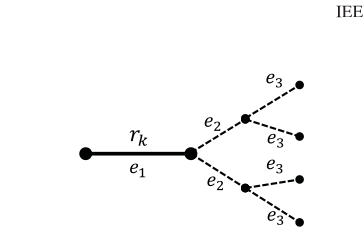
\includegraphics[]{figures/prediction_tree_omm.png}
    \caption{Contoh \textit{prediction} tree dari algoritma OMM-MHT.}
    \label{fig:prediction-tree-omm}
\end{figure}




\begin{algorithm}
\caption{Online Map-Matching dengan menggunakan Multi Hypothesis Technique} 
\label{alg:omm-mht}
\resizebox{\textwidth}{!}{%
\begin{minipage}{\textwidth}
\scriptsize
\begin{algorithmic}[1]
\setstretch{0.9}
    \Procedure{OnlineMapMatchingMHT}{$G(V,E),g_{1:k},\Delta t_{1:k}$}
        \State $C \gets \{c\mid c.w=c.e.l, c.e \in E, dist(g_1,c.e)<L_C\}$
        \State $\overline{v} \gets g_1.v$
        \State $\sigma_v \gets \sigma_v$
        \For {$k=1 \textbf{ to }K$}
            \If {$k>1$}
                \State $C_{new} \gets \emptyset$
                \For {$\textbf{all } c \in C$} \Comment{prediksi}
                    \State $\tau \gets \{c.e\}$
                    \State $p_\tau\gets 1$ \Comment{menghitung $p(\tau)$}
                    \State $h_{pre} \gets 1$
                    \State $C_{new} \leftarrow$ \Call{Recur}{$C_{new},c.w,\tau,p_\tau,\overline{v},\sigma_v,\Delta t_{k-1}, h_{pre}$}
                \EndFor
                \State $C\leftarrow C_{new}$
                \State $\overline{v},\sigma_v\leftarrow KalmanFilter(\overline{v},\sigma_v,g_k.v)$
            \EndIf

            \For{$\textbf{all }c\in C$} \Comment{filtering}
                \State $c.w\leftarrow \frac{c.w.ObservationProb(g_k,c)}{\sum_{c'\in C}c'.w.ObservationProb(g_k,c')}$ \Comment{menghitung posterior $p(r_{k+1}\mid g_{1:k+1})$}
            \EndFor
            \State $\{c\mid c\in C, c.w>L_u\}$
            \State $r_k\leftarrow (\arg \max_{c\in C} c.w).e$
            \State \textbf{output } $r_k$
        \EndFor
    \EndProcedure

    \Procedure{Recur}{$C_{new},w,\tau,p_\tau,\overline{v},\sigma_v,\Delta t_{k-1}, \text{ dan } h_{pre}$}
        \State $h_{new}\leftarrow h(\tau,\overline{v},\sigma_v,\Delta t_{k-1})$ \Comment{menghitung $h(\tau_{1:n},\overline{v}_k,\sigma_{v,k},\Delta t_k)$}
        \If {$w \cdot p_\tau \cdot h_{new}>L_p$}
            \State $\mathcal{E}_{next} \gets \{e_{next}\mid e_{next}\in E, e_{next}.start=\tau.last.end\}$
            \For {$\textbf{all } e_{next}\in \mathcal{E}_{next}$}
                \State $\tau'\gets \{\tau\rightarrow\ e_{next}\}$
                \State $p_{\tau}' \gets p_\tau \cdot p(\tau.last\rightarrow e_{next})$ \Comment{menghitung probabilitas $p(e_{\tau.last}\rightarrow e_{next})$}
                \State $h'_{pre}\gets h_{new}$ \Comment{menghitung $h(\tau_{1:n-1},\overline{v}_k,\sigma_{v,k},\Delta t_k)$}
                \State $C_{new}\gets Recur(C_{new},w,\tau',p_{\tau}',\overline{v},\sigma_v,\Delta t_{k-1}, h'_{pre})$
            \EndFor
        \EndIf 
        \State $w' \gets w\cdot p_{\tau}\cdot (h_{pre}-h_{new})$ \Comment{menghitung $p(r_{k+1}\mid r_k)$}
        \State $c_{new}\gets C_{new}.Find(c_{new}\mid c_{new}.e=\tau .last)$
        \If{$c_{new}\neq null$}
            \State $c_{new}.w=c_{new}.w+w'$
        \Else 
            \State $C_{new}\gets C_{new}\cup (\tau.last, w')$
        \EndIf
        \State \textbf{return} $C_{new}$
    \EndProcedure
        
    \Procedure{KalmanFilter}{$\overline{v}, \sigma_v, g_k.v$}
        \State $\overline{v}_{k}=\overline{v}_{k-1}$ \Comment{prediction}
        \State $\sigma_{v,k}=\sqrt{\sigma^2_{v,k-1}+ \sigma^2_{a}\Delta t^2_{k-1}}$
        \State $\overline{v} = \frac{\sigma_v^2 \overline{v}_{k}+\sigma^2_{v,k} g_k.v} {\sigma_v^2+\sigma_{v,k}^2}$\Comment{filtering}
        \State $\sigma_{v,k} =\sqrt{(\sigma^{-2}_v + \sigma^{-2}_{v,k})^{-1}}$
    \EndProcedure
\end{algorithmic}
\end{minipage}%
}
\end{algorithm}



